\newpage
\section{Spesefikke anleggs forskjeller}
\thispagestyle{fancy}

Sjølv om Sande reiseanlegg anvender \gls{SBR}-teknologi så er det enkle spesefikke
punkter der dette reiseanlegget avviker ifrå normen. 
Sande reinseanlegg bruker eksempelvis ein spesiel form for slambehandling sett i norsk perspektiv.

Vanleg slambehandling i Noreg er oppsamling av slammet i tanker som handterast og tømmast av lokale etater.
På Sande blir ikkje slammet lagra, men jamnlig spreid ut over eit designert område. På dette området er
det planta siv som skal ta opp slammet og det resterande vatnet blir naturleg filtrert og drenert.
Desse områda kallast sivbed.

Sivbeda er konstruert med fleire dreneringslag som gjer at resterande vatn skiljast ut i designerte soner.
Her kan desse handterast vidare etter ønska behov. 
Grunna denne slambehandlingsmetoden er det på Sande reiseanlegg heller slamfjerning frå reaktor
i reaksjonsfasen. Dette blir gjort for å ha mindre konsentrert slam.

Sande reiseanlegg har fire sivbed med kombinert størrelse på 676 kvadratmeter, som står på utsida av reiseanlegget.


\begin{figure}[htbp]
    \centering
    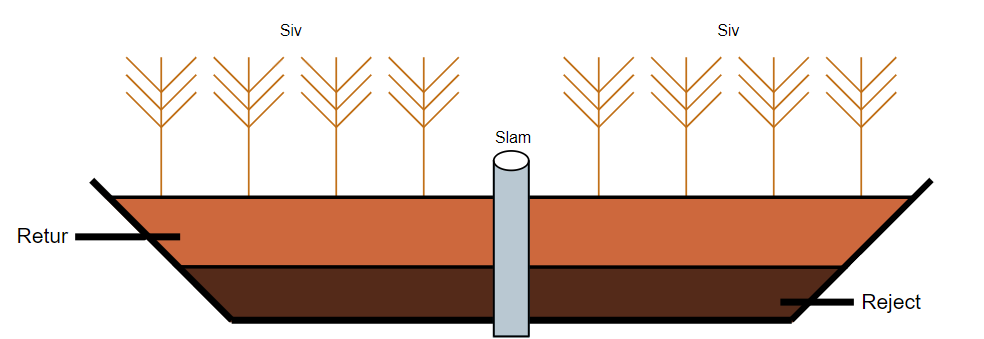
\includegraphics[width=1\textwidth]{Figurar/Sivbed.png}
    \caption{Illustrasjon sivbed}\label{fig:HMI}
\end{figure}


\newpage

Vatnet frå desse forskjellige dreneringslaga blir samla til eit pumpehus/komme.
Dette pumpehuset står ca femti meter ifrå sjølve reinseanlegget og er utstyrt med to pumper og nokre nivåbrytarar.
Pumpekommen er delt i to og skiller på vatnet som kjem ifrå dei forskjellige dreneringslaga. \newline
På Sande reiseanlegg er djupaste dreneringssona klassifisert som reinsa vatn (sivbed reject) og blir sendt ut til resepient.
Den øvre dreneringssona er forsatt klassifisert som skitten og blir returnert til mottakstanken.

\begin{figure}[htbp]
    \centering
    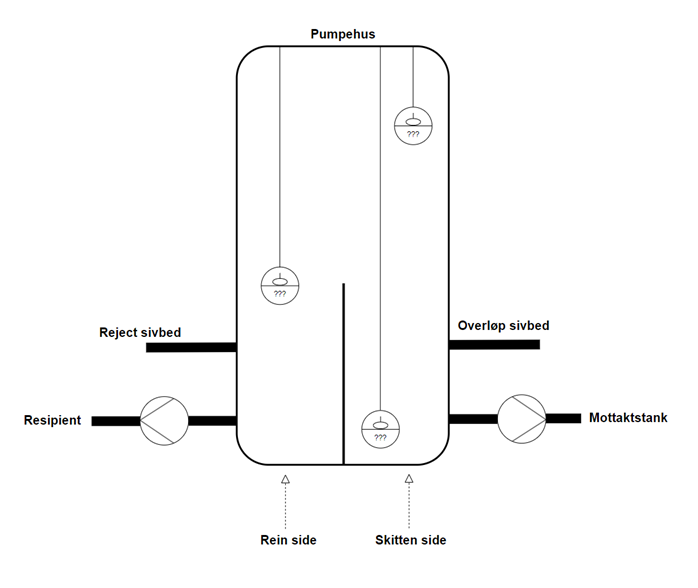
\includegraphics[width=1\textwidth]{Figurar/Pumpehus.png}
    \caption{P\&ID pumpehus}\label{fig:HMI}
\end{figure}

\newpage



